\chapter{Kontext}

\section{Testování softwaru při vývoji}
Při vývoji softwaru je vhodné vyvíjený software neustále testovat. Software lze testovat
více způsoby, ale cílem testů je vždy otestovat některý z~důležitých kvalitativních
atributů, jako je například korektnost nebo výkon. Testování výkonu není dnes při vývoji softwaru příliš obvyklé. \cite[]{unitTestingPerformanceSurvey}

Pro testování korektnosti se obvykle používají unit testy. Jedná se většinou o~krátké testovací
funkce, které kontrolují, jestli se testovaný kód chová požadovaným způsobem. Zjišťují tedy, jestli
kód na zadaný vstup vrátí očekávaný výstup. Ke~kódu, který není aktuálně vyvíjen, se obvykle nemění
ani unit testy. Když se mění části kódu kolem již takto hotové části, tak unit testy stále průběžně sledují
korektnost tohoto již hotového kódu. Zdali je kód korektní se pomocí unit testů zjistí velmi jednoduše.
Kód je korektní, pokud vrátil očekávaný výstup a~pokrytí kódu unit testy je dostatečné.

\section{Průběžná integrace}
Při vývoji softwaru se často používají nástroje pro automatizování některých činností.
Obvykle se automatizují činnosti jako jsou správa verzí, spouštění testů a jejich vyhodnocování.

Pro správu verzí při vývoji softwaru se obvykle používá nástroj Git.
Git je vhodný i~pro práci ve velkých týmech.
Umožňuje totiž členění projektu do větví. Každá větev je vhodná pro vývoj samostatné části aplikace.
Následným spojováním větví pak dochází k propojení větších funkčních celků aplikace, které byly vyvinuty v~jednotlivých větvích.
Nástroj si formou pamatování si změn udržuje přehled o~průběžných verzích a~provedených změnách.
Nástroj je možné ovládat jednoduchými příkazy z~příkazové řádky.
Je to tedy nástroj, který je možné ovládat ze skriptů.

Nástroj Git umí jednoduše zprostředkovat průběžnou integraci (continuous integration). Průběžná integrace umožňuje uživateli dělat automatizované
kroky při nahrávání nových verzí do~větve nebo při spojování větví. Při průběžné integraci tedy jde o~spouštění
skriptu při některé ze zmíněných událostí. V rámci průběžné integrace je možné testovat software pomocí unit testů
i~benchmarků pro měření výkonu. Dále je možné použít jakékoli jiné příkazy příkazové řádky.
Do průběžné integrace je tedy možné jednoduše zapojit téměř jakoukoli konzolovou aplikaci.
Při selhání skriptu, když skončí s nenulovým exit kódem, je možné změny neintegrovat.
Tímto způsobem je možné zamezit integraci chybného kódu.

\section{Měření výkonu}

Testování výkonu obvykle probíhá tak, že se použije nějaký vhodný měřící framework.
Obvyklé frameworky pro měření výkonu mají vlastní pravidla, jak se mají označit metody, které
se mají měřit. Tyto frameworky umožňují měřit výkon softwaru podle různých metrik. Mezi tyto metriky
se řadí čas, propustnost a~například spotřeba paměti. Výsledky měření umí frameworky obvykle zaznamenat jak do~strojově
čitelného formátu, tak do formátu čitelného pro člověka.

V~dalších podkapitolách jsou uvedeny příklady měřících frameworků pro jazyky C\# a~Java.
Z~uvedených příkladů bude patrné, že tyto frameworky samy o~sobě nemohou poskytnout informace o~změně výkonu.
Neuchovávají totiž informace o měření jiné verze softwaru, než té měřené. Jak již bylo v úvodu naznačeno,
výsledky měření je nutné porovnat s~výsledky měření jiné verze softwaru. Zmíněné nástroje toto neumí,
ale pro samotné měření výkonu jsou velmi vhodné.

\subsection{BenchmarkDotNet}

BenchmarkDotNet je framework určený k~měření výkonu programů na~platformě .NET. V~důsledku
toho, že měří programy na platformě .NET, je schopen měřit výkon programů napsaných
v~programovacích jazycích C\#, F\# a~Visual Basic. Podrobnosti o~tomto měřícím frameworku
je možné nalézt v~dokumentaci \cite[]{benchmarkDotNet}.

Při~měření výkonu pomocí BenchmarkDotNet se měřené hodnoty vypisují na~standardní výstup
včetně konečného shrnutí. Mimo standardní výstup se ještě výsledky měření ukládají
do~strojově zpracovatelných formátů, jako je například JSON nebo CSV.

Výstupem měření výkonu programu v~jazyce C\# pomocí frameworku BenchmarkDotNet jsou již statisticky zpracované hodnoty.
Aby bylo možné sledovat jednotlivé naměřené hodnoty, je nutné zvolit již při~psaní testů správný
exportér, který tuto funkci podporuje.

\begin{figure}[!ht]
    \centering
    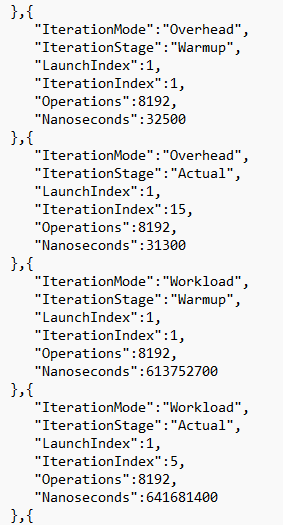
\includegraphics[width=0.3\textwidth]{../img/BenchmarkDotNET-modes.png}
    \caption{Struktura výsledků měření frameworku BenchmarkDotNET}
\end{figure}

BenchmarkDotNet je možné nakonfigurovat tak, aby se v~souboru s~výsledky nacházely podrobnosti o~prostředí, jako je operační systém,
verze platformy .NET, jméno, typ a~parametry procesoru. Dále aby se v~souboru s~výsledky nacházely
výsledky jednotlivých provedených měření. Výsledek měření u~sebe má informaci o~jméně
testovací metody, zpracované statistické údaje a~naměřené hodnoty z~různých módů a~iterací měření.
Konkrétní příklad toho, jak vypadají módy a~iterace měření se nachází na obrázku 2.1.
Názvy módů a~iterací mají intuitivní názvy, takže je z~nich poznat, kdy se ještě probíhá
překlad, a~kdy už se měří plně přeložený kód. C\# je totiž jazyk kompilovaný metodou JIT,
a~proto kód není přeložen se všemi optimalizacemi hned na začátku, tudíž je nutné měřit
více iterací, než se kód plně přeloží.

\subsection{JMH (Java Microbenchmark Harness)}

JMH je framework pro měření výkonu, který umožňuje pomocí anotací definovat výkonnostní testy
pro programy v~jazyce Java. Z~průzkumu \cite[]{unitTestingPerformanceSurvey} vyplývá, že se jedná o~nejpoužívanější framework
pro měření výkonu pro projekty vyvíjené v jazyce Java.

JMH obdobně jako BenchmarkDotNet poskytuje výsledek měření jako tabulku na standardní výstup.
Dále poskytuje výstup v~podobě strojově zpracovatelných formátů, jako jsou například XML
nebo JSON. O~výstup v~této podobě je nutné zažádat pomocí argumentů na~příkazové řádce při
spouštění měření. Další podrobnosti o~frameworku JMH je možné nalézt v~dokumentaci \cite[]{jmh}.

\begin{figure}[!ht]
    \centering
    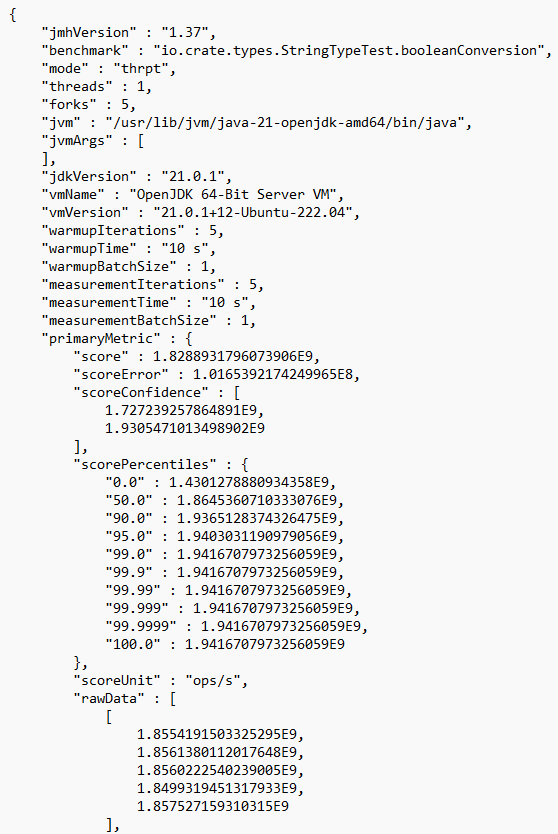
\includegraphics[width=0.6\textwidth]{../img/JMH-example.png}
    \caption{Struktura výsledků měření frameworku JMH}
\end{figure}

Ve výstupním souboru měření pomocí JMH lze nalézt informace o~stroji na~kterém probíhalo měření.
Jedná se především o~název stroje a~verzi operačního systému. Dále zde lze nalézt verzi Javy,
ve~které probíhalo měření. V~souboru je možné vidět také ostatní parametry měření, jako je
zahřívací doba a~počet zahřívacích iterací. Zahřívací iterace jsou zde uvedeny, protože Java
je stejně jako C\# jazyk kompilovaný metodou JIT, a~tak je také nutné měřit více iterací, než se kód
plně přeloží se všemi optimalizacemi.

Jednotlivé naměřené hodnoty jsou ve výstupním souboru dostupné i~ve~výchozím nastavení JMH.
Naměřené hodnoty nejsou bezrozměrná čísla, ale jsou doplněny i~o~fyzikální jednotku,
kterou naměřená hodnota reprezentuje. Pro~každý běh (fork), přičemž běhů může být v~jednom
spuštění JMH více, se~objeví jedna sada měřených hodnot u~položky \lstinline|rawData|.

\section{Scénář}

Mějme programátora, který vytváří softwarové dílo. Mezi dobré programovací zásady patří udržovat kvalitu kódu
hned od začátku vývoje. Programátor tedy podle dobrých zásad začne používat verzovací nástroj.
Tento samotný nástroj pro udržování kvality kódu nestačí. Umožní ale programátorovi použít průběžnou integraci.

Programátor dále podle zvyku začne psát unit testy pro vytvářený kód. Unit testy mu pomohou udržovat korektnost kódu.
Korektnost je jedním z aspektů kvality kódu. Aby mu unit testy pomohly udržovat kvalitu kódu, musí dobře pokrývat kód.
Výhodou unit testovacích frameworků je jejich snadné zapojení do průběžné integrace. Programátor je tedy začne
tímto způsobem spouštět s každou novou verzí.

Dalším z~aspektů kvality kódu, které by chtěl udržovat je výkon. Programátor s~využitím nějakého frameworku pro~měření výkonu začne měřit výkon svého kódu.
Měření výkonu se trochu podobá unit testům. U~měřících frameworků jako je BenchmarkDotNET nebo JMH se vytvoří specializované měřící metody,
které se podobají unit testovacím metodám z~unit testovacích frameworků jako je například JUnit.
Tyto měřící metody, ale změří pouze číslo a~jednotku, která nevypovídá o~změně výkonu oproti jiné verzi.
Pokud chce programátor výkon udržovat potřebuje vyhodnotit právě tuto změnu.

Programátor tedy musí vzít výsledky měření aktuální verze a výsledky měření referenční verze vůči které chce
změnu výkonu vyhodnocovat a sám výsledky porovnat. Porovnání výsledků měření nemusí být možné pouhým pohledem
na sady číselných dat. Pravděpodobně si budou hodnoty hodnoty obou sad podobné. Obzvlášť pokud změna bude příliš málo výrazná.
Proto by programátor musel nejprve číselná data nějakým způsobem sám zpracovat. Ze zpracovaných dat by pak pro každou měřenou metodu
kódu musel vyhodnotit zdali došlo k výrazné změně výkonu, které by se měl dále věnovat.

Cílem této práce je vytvořit nástroj, který by programátorovi pomohl s vyhodnocováním změn výkonu.
Nástroj by mělo být možné co nejjednodušeji zapojit do průběžné integrace. Jeho výstup by se měl co nejvíce podobat
výstupu unit testovacích frameworků. Měl by tedy poskytovat výstup ve strojově čitelném formátu, ale také ve formátu
čitelném pro člověka. Očekává se, že nástroj bude hlásit výrazné změny výkonu mezi dvěma verzemi a~že bude nezávislý
na použitém měřícím frameworku.





